\documentclass{ecai}
\usepackage{times}
\usepackage{graphicx}
\usepackage{latexsym}
\usepackage{xspace}
\usepackage{hyperref}
\usepackage{amssymb}
\usepackage{algorithm}
\usepackage[noend]{algpseudocode}
\usepackage[numbers]{natbib}
\usepackage{notoccite}
\usepackage{framed}
\usepackage{amsmath}

\usepackage[dvipsnames]{xcolor}
\newcommand{\sergey}[1]{\textcolor{magenta}{{\sc Sergey:} #1}\xspace}
\newcommand{\samuel}[1]{\textcolor{green}{{\sc Samuel:} #1}\xspace}

\newcommand{\constraints}{\ensuremath{\mathcal{C}}\xspace}
\newcommand{\format}[1]{\textit{#1}\xspace}
\newcommand{\generategroups}{\format{generateAssignments}}
\newcommand{\extractgroups}{\format{extractGroups}}
\newcommand{\extracttables}{\format{extractTables}}
\newcommand{\learnconstraints}{\format{learnConstraints}}
\newcommand{\findassignment}{\format{findSolutions}}
\newcommand{\postprocess}{\format{pruneRedundant}}
\newcommand{\constrainttorder}{\format{orderedConstraints}}


\newcommand{\CName}{Name\xspace}
\newcommand{\CSignature}{Signature\xspace}
\newcommand{\CFunction}{Function\xspace}
\newcommand{\dependencies}{\ensuremath{\mathcal{D}}\xspace}
\newcommand{\groups}{\ensuremath{\mathcal{G}}\xspace}

\newcommand{\range}[3]{\ensuremath{#1[#2,#3]}}
\newcommand{\rangeto}[2]{#1{:}#2}
\newcommand{\rangeall}{:}

\newcommand{\ecrank}[2]{\ensuremath{#1 = \mathit{RANK}(#2)}}

%%\ecaisubmission   % inserts page numbers. Use only for submission of paper.
                  % Do NOT use for camera-ready version of paper.

\begin{document}

\title{Tabular Constraint Learning}

\author{Name1 Surname1 \and Name2 Surname2 \and Name3 Surname3 \institute{KU Leuven, Belgium, email: firstname.lastname@kuleuven} }

\maketitle

\begin{abstract}
  abstract
\end{abstract}
\section{Introduction}
Imagine you have received a CSV file. Upon examining the content it becomes fairly clear it was made in Excel. Even the names of the fields such as Total or Avg indicated the usage of the standard functions. Having a closer look, you could deduce the functional dependencies in the table that look as in Figure \ref{fig:main_example}. Provided that a spreadsheet and the numbers in it are small, and dependencies are not complicated, one can examine the spreadsheet and find all connections. But wouldn't it be good to do it automatically?

This brings us to the \textbf{key question}:\\
Can we discover or reconstruct structural relations in flat tabular spreadsheet data? [in a general way that allows declarative specification of constraints to discover]\\

Of course, it is stated semi-informally here, but it already allows us to provide an intuition on the task. We know that often people work in Excel with ranges, e.g. if we look at the Table 1  and at the first row in the Table 2 in Figure \ref{fig:main_example}, it is clear that one could have selected the first columns, clicked on the \textit{SUM} function and then just used the drag fill handle to apply the formula to the other columns. Similarly, that would work for the second (\textit{Average}), third (\textit{Min})  and forth (\textit{Max}) rows in Table 2. I.e., all operations are vectorized and make use of the standard Excel functions. 

It is not hard to see that computation goes not only in columns but in rows as well: if we sum the values in Table 1 in the first row in all four quarters, we would obtain the seventh column in Table 1. That gives us already a hint how this problem is different from the standard data mining settings, when the data is in rows and variables are in columns. Here everything is mixed, some values are missing in the results, some missing the arguments, even a header might have missing values. The data is relational on one hand, since we have multiple table with relationships between them. And on the other hand, the data is numeric, since people tend to use spreadsheets for financial and accounting computations, which is heavily numeric.

\sergey{we need to incorporate the motivation part like error checking and autocompletion in the intro}

\sergey{bullet points for Luc and Tias to rework introduction}\\
\textbf{Motivation}:
\samuel{Suggest better table layouts / formula translation}
\begin{itemize}
  \item File generated from model, model got lost, need to reconstruct
  \item Constraint programming is hard - is Excel hard?
  \item Avoid manual analysis, provide selection of constraints
  \item Error checking
  \item Completion, gain speed and insights (Complicated constraints, also complicated to verify, too much output)
\end{itemize}

\textbf{Novelty:}
\begin{itemize}
  \item Unsupervised setting (contrary to flashfill, etc)
  \item Numeric, different constraints (contrary to single textual function solution in flashfill, etc)
  \item Data format (2D) -- data is no longer in rows like a classic ML or DM settings
  \item Declarative, general / modular, stacking of constraint problems 
\end{itemize}

\sergey{need to elaborate the example here: like in a story} 

\begin{figure*}[tbh]
  \begin{center}
    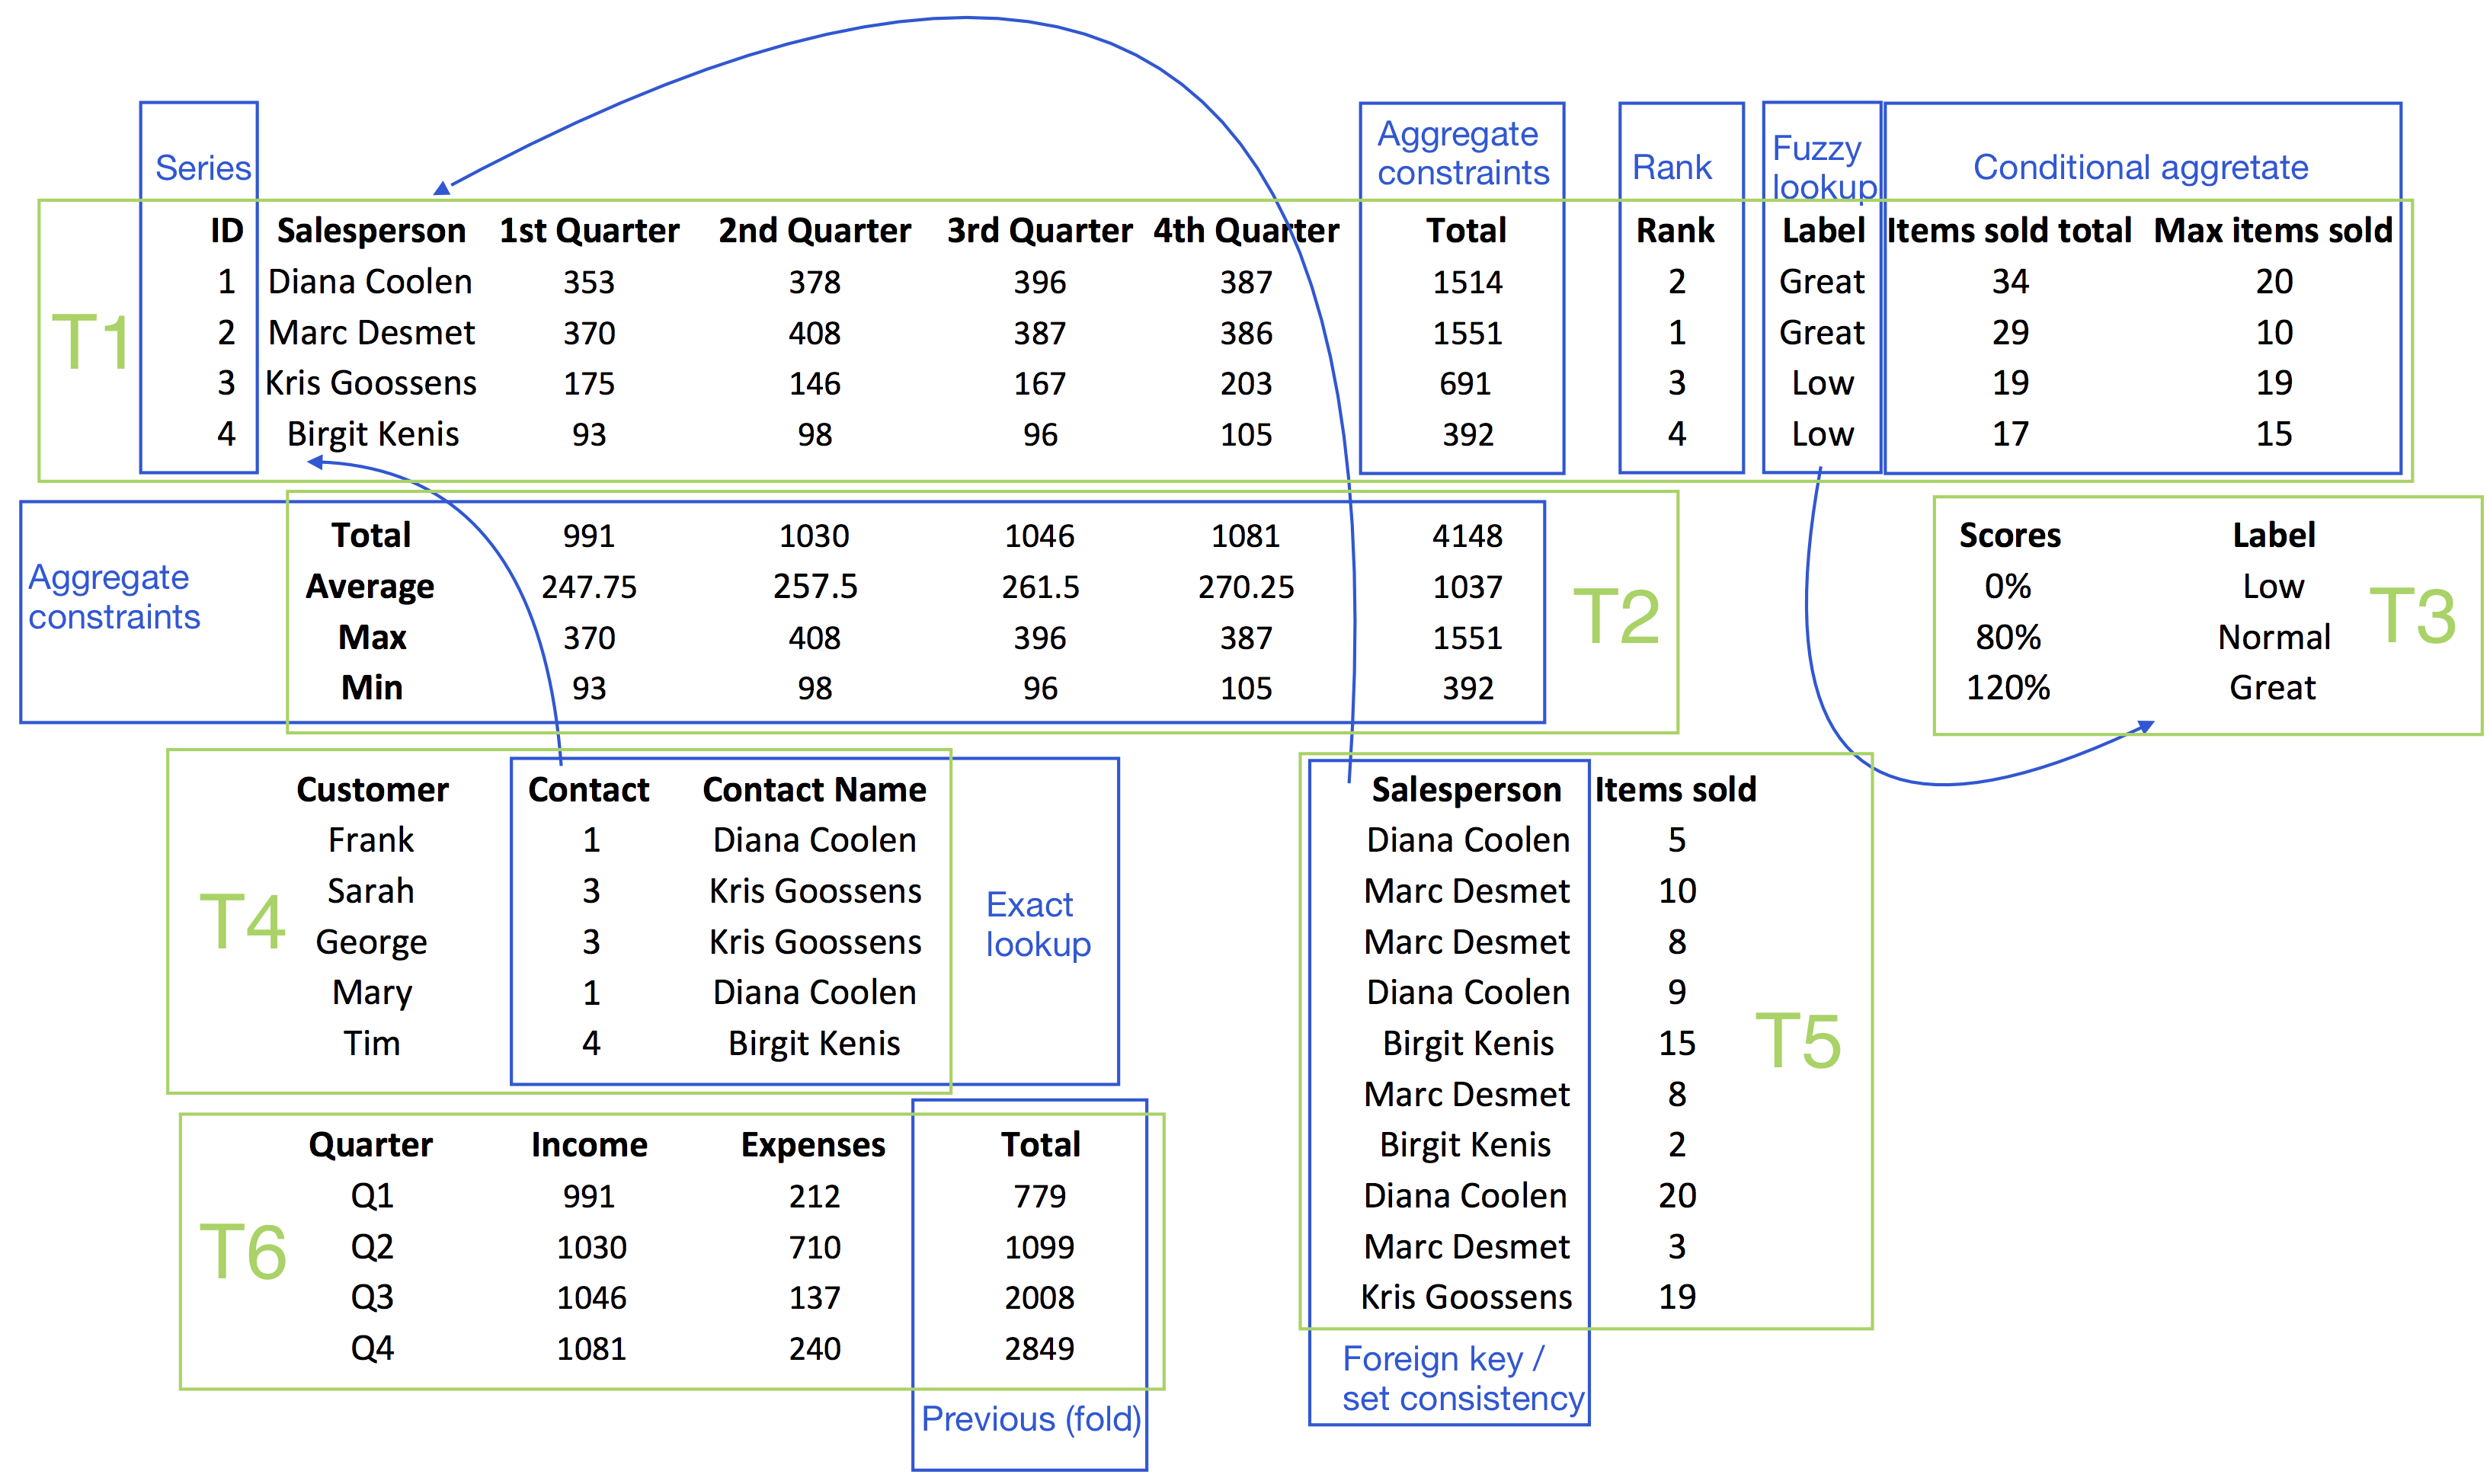
\includegraphics[width=0.75\textwidth]{figures/Demo.png}
  \end{center}
  \vspace{-10pt}
  \caption{An example of constraint reconstruction (in blue) with indicated groups (in green)}
  \label{fig:main_example}
\end{figure*}

\section{Formalization}

\samuel{Explain concepts on example}
\subsection{Groups, Type-consistency and Constraints}
In this work we distinguish the following types of data: numeric and textual. The numeric type has two subtypes: integers and floats. We also consider the special element called \textit{None}, which has two types: numeric and textual. A set is called \textit{type-consistent} iff all elements are either numeric or textual. Certain constraints, such as \textit{rank} or \textit{series}, make use of the numeric sub-types by requiring its arguments to be integers.

A \textit{vector} is either a column or a row that is type-consistent. If a vector is a row (column), we say that it has a \textit{row} (\textit{column}) orientation. A \textit{group} is a subrange of vectors with the same orientation in a table. We use the following notation to refer to a row (column) group $G$ in a table $T$ with rows (columns) ranging from $a$ to $b$: $G = T[a{:}b,:]$ ($G = T[{:},a{:}b]$), where $a,b$ are natural numbers. We denote as the \textit{length} of a row (column) group $G$, written as \textit{length(G)}, the number of its columns (rows). We call a group $G$ \textit{numeric} (\textit{textual}, etc), written as \textit{numeric(G)}, if its vectors contain numeric (textual, etc) elements.

An \textit{Excel constraint} is a triple \textit{(\CName, \CSignature, \CFunction)}. Let us elaborate on each of them. \textit{\CName} is the textual name of the constraint together with its variable names. \textit{\CSignature} is a set of constraints specifying the properties of the group assignments, corresponding to the variables in \CName, such as their types, e.g., requiring them to be integers or constraining the sizes, e.g. the length of vectors in the arguments must be equal. These are constraints on the group meta-information not on the actual group content. \textit{\CFunction} is a set of constraints specifying that the data in the subgroups satisfies the function. For example, an excel constraint \textit{rank} has \CName \textit{Y = RANK(X)}, where $X$ and $Y$ are the variables; its \CSignature is: the group $G_X$ (associated with X) is numeric, $G_Y$ is integer and the length of vectors in $G_X$ is the same as in $G_Y$; its \CFunction is the following constraint: a pair of vectors $X,Y$ is a solution iff $X \in G_X, Y \in G_Y$ and each value in $X$ has the rank (possibly with ties) specified in $Y$.

\samuel{2nd problem statement (from approach), remove EQUAL}

A \textit{tabular solution} $S$ to an Excel constraint $C$ is a tuple $(X_1, \dots, X_n)$ where $n$ is the number of variables in $C$ and each $X_i$ is a subgroup in \groups, such that $(X_1,\dots,X_n)$ satisfies both the \CSignature and \CFunction of the constraint $C$.

\section{Problem Statement}
In the previous section we introduced the problem of tabular constraint learning informally using the example in Figure \ref{fig:main_example}. Here we formalize the statement in terms of Excel constraints and group assignments as follows: 

\begin{minipage}[c]{14em}
  \vspace{5pt}
  \begin{tabular}{ll}
    \multicolumn{2}{l}{{\textbf{Tabular Constraint Learning Problem}}}\\
    \vspace{-4pt}
    &\\
    \textbf{Given:}& the set of all groups $\groups$ and of Excel constraints $\constraints$\\
    \textbf{Find:}&  all tabular solution $S$ in \groups for each constraint $c$ \constraints \\ 
  \end{tabular}
  \vspace{6pt}
\end{minipage}

  The key observation here is that essentially the problem is a constraint enumeration problem, where each constraint is independent. This property comes from fact that in Excel each formula is applied based on the existing data in the cells. This allows learning constraints independently of each other by examining constraint satisfaction on the groups.


  In theory each constraint is independent and equally useful. In practice, however, things are different. Assume that for some $X$ both \textit{series(X)} and \textit{alldifferent(X)} hold. From a user's perspective the last solution is useless, since he or she already knows that series constraint implies alldifferent constraint. To capture this condensed representation \cite{condensed} of solutions, we have introduced a specificity (generality) order between constraints, which is depicted using solid (dashed) arrows in Figure \ref{fig:learning_order}. This matters from implementation perspective as well, if we discovered that $X$ is a not permutation, then $X$ should not be tested for the series constraint at all. A solid lines from $C_1$ to $C_2$ indicates that $C_2$ is \textit{more specific} than $C_1$ and if $X$ is not a solution to $C_1$, then it is not a solution to $C_2$. A dashed arrow from $C_1$ to $C_2$ indicates that $C_1$ is \textit{a more specific} constraint than $C_2$ and therefore if $X$ is a solution for $C_1$ it should not be tested for $C_2$.

We call a tabular solution $S$ to a constraint $C$ \textit{the most specific} wrt \dependencies, iff there is no other constraint $C'$ for which $S$ is a solution and $C'$ is more specific in \dependencies.


Let us introduce the version of tabular constraint learning that takes into account the specificity relation between constraints.

\begin{minipage}[c]{14em}
  \vspace{5pt}
  \begin{tabular}{ll}
    \multicolumn{2}{l}{{\textbf{Condensed Tabular Constraint Learning Problem}}}\\
    \vspace{-4pt}
    &\\
    \textbf{Given:}& the set of all groups $\groups$ and of Excel constraints $\constraints$,\\ 
    & a constraint specificity DAG \dependencies \\
    \textbf{Find:}& all the most specific wrt \dependencies solutions $S$ in \groups\\ 
    & for each $c$ in \constraints \\
  \end{tabular}
  \vspace{6pt}
\end{minipage}

This version explicitly takes into account the specificity of the constraints and invalidates some of the solutions that are entailed by the tabular other solutions.

\section{Approach to Tabular Constraint Learning}
As we have seen the statement before assumes the set of groups to be given. It is often, however, not the case and a possible approach is to extract the groups from the CSV file directly. In our system, we have implement the group construction step using the type-consistency check. \sergey{Samuel, we need details here, I think} In general, separating data from a header is a task on its own  \cite{header} and goes beyond the scope of this paper. 

Another solution to the group extraction problem is to make it interactive, when a user can select the groups in the spreadsheet or correct automatically generated groups. We regard this approach to be a possible future direction in the system development. Later in the paper we assume the groups to be given.

Now we describe how the problem of Condensed Tabular Constraint Learning can be solved. The algorithm mimics the structure of the problem in the following way: first we need to order constraints in the order of specificity, then for each constraint we need to generate possible candidate groups, and in the next step we find the subgroups satisfying the constrain. After an iteration we accumulate all solutions and proceed to the next constraint.

\begin{algorithm}[thb]
  \begin{algorithmic}
    \footnotesize
    \State \textbf{Input:} $\groups$ -- groups, $\constraints$ -- Excel constraints, \dependencies -- dependency graph 
    \State \textbf{Output:} $S$ -- learned constraints with their satisfaction assignments
    \State $S \gets \emptyset$ \Comment{The set of solutions}
  \For{$c \in \constrainttorder(\constraints,\dependencies)$} 
  \State $v_1, ..., v_n =$ variables of $c$ 
    \For{$v_1{:}~G_1, \dots, v_n{:}~G_n \in \generategroups(c, G, S, \dependencies)$}
      \State $S \gets S \cup \findassignment(c, v_1{:}~G_1, \dots, v_n{:}~G_n, S, \dependencies)$
    \EndFor
  \EndFor\\
\Return $S$
\end{algorithmic}
\caption{Tabular constraint learning}
\label{algo:tcl}
\end{algorithm}
Essentially, our Algorithm \ref{algo:tcl} has three steps: constraint ordering, candidate group generation and subgroup satisfaction search, which is in line with the ``generate-and-test'' paradigm that is well-known in AI \cite{whaisasp}. Let us elaborate on each step in detail. 

\samuel{Running example (RANK?)}
\paragraph{Constraint ordering} $\constrainttorder(\constraints,\dependencies)$ uses the DAG \dependencies in Figure \ref{fig:learning_order} in the following way: all constraints are generated in the topological order of \dependencies. Also, if there is a solid edge from $C_1$ to $C_2$, and $X$ is not a solution to $C_1$, then $X$ is not generated as a candidate group for $C_2$. If there is a dashed edge from $C_1$ to $C_2$ and $X$ is a solution to $C_1$, then $X$ is not generated as a candidate group for $C_2$.

\paragraph{Candidate group generation} $\generategroups(\textit{Constraint,GroupSet,Solutions})$ is the function generating tuples of groups that are legitimate solution candidates e.g., $X,Y$ are variables of \textit{Y = RANK(X)} and $X,Y$ satisfy the constraints from \CSignature above. Essentially, the group generation step is a constraint satisfaction problem associated with the specific constraint. However, many constraints have the same candidate generation procedures, e.g., sum, min, max, avg, count, etc.

\paragraph{Subgroup satisfaction search} $\findassignment(\textit{Constraint,Candidates,Solutions})$ is the function looking for the subsets of vectors in the candidates satisfying the constraint. If multiple subsets satisfy the constraint, a maximal is selected. If $G_1,G_2$, associated with the variables $X,Y$ in the constraint \textit{Y = RANK(X)}, are candidates, then \findassignment selects a single vector $y$ in $G_2$ and a single vector $x$ in $G_1$ such that $x$ is ranked by $y$. For example, in Figure \ref{fig:main_example} the group $G = T_1[{:},3{:}8]$ serves as $X$ and $Y$ and $x$ can be picked as $T_1[{:},7]$ and $y$ would be $T_1[{:},8]$.

\samuel{Expand aggregates to max within group, tweak groups if necessary}
\sergey{[23:32:21] Samuel Kolb: And the motivation is that you can make the group smaller if you want to exclude a column from the aggregate that does not belong in it but accidentally gets included}

\paragraph{Implementation note} Essentially for each constraint both \generategroups and \findassignment are separate constraint satisfaction problems. Hence, it is natural to solve them using declarative solvers. Even though each is a separate constraint problem, they are variations of each other and can be modeled using similar techniques. It also makes an extension of the system easy, we can solve new variations by adding, removing or modifying constraints from a similar constraint satisfaction problem. Furthermore, the declarative languages such as ASP \cite{whaisasp} and Minizinc \cite{minizinc} provide primitives that make modeling transparent and generic.

Our system internally supports ASP (using Clingo 4.5.4 \cite{clingo}), Minizinc (Gecode-backend 2.0.2 \cite{minizinc}) and a native python CSP solver \cite{python_constraint}. All the constraints mentored in the paper can be run purely in the internal python engine without any external software. The future versions of the system will provide user interfaces to the ASP, Minizinc and Python-Constraint languages.

\subsection{Constraints}
As emphasized before, the set of Excel constraints has a partial order in which they should be learned. For certain constraints this order does not matter, such as \textit{rank} or \textit{product}. For many others they have to be learned in the order, which is specified as a DAG in Figure \ref{fig:learning_order} (if a constraint is not in the graph, it is independent). This figure also specifies a potential parallelization of the computation, since each connected component is independent of the others.


\begin{figure}[htb]
  \centering
  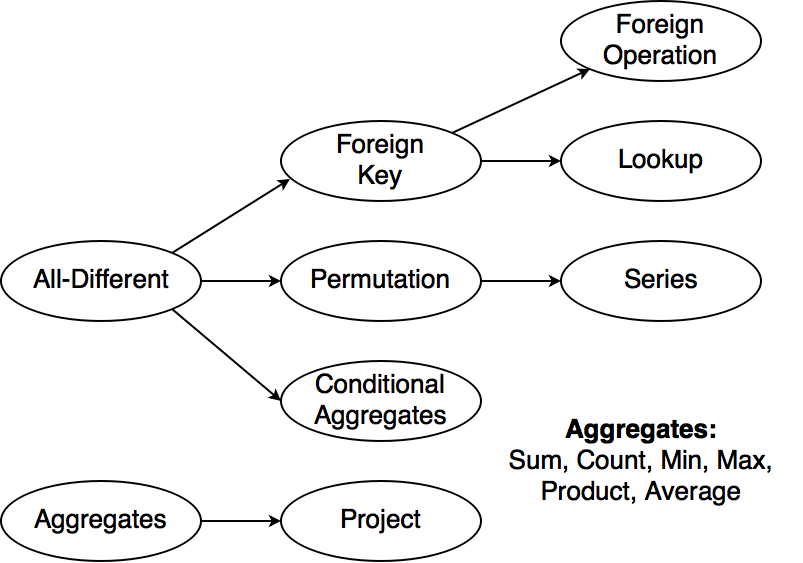
\includegraphics[width=0.20\textwidth]{figures/constraint_dependency.png}
  \caption{Constraint Learning Order. The solid arrows indicate a specificity order, i.e., \textit{permutation} $\rightarrow$ \textit{series} means that the series constraint is more specific than permutation. The dashed arrows indicate an inverse construction order, \textit{project} $\dashrightarrow$ \textit{aggregates} means the project constraint is more specific than aggregates. \sergey{Samuel,  can you give an explanation why we keep both arrow and how it is internally motivated?}}
  \label{fig:learning_order}
\end{figure}


\newcommand{\numeric}{\format{numeric}}
\newcommand{\textual}{\format{textual}}
\newcommand{\integer}{\format{integer}}
\newcommand{\length}{\format{length}}
\newcommand{\nat}{\mathcal{N}}

\begin{table*}
  \centering
  \begin{tabular}{lcc}
    \textbf{\CName} & \textbf{\CSignature} & \textbf{\CFunction}\\
    ALLDIFFERENT(X) & & \\
    X = Y & & \\
    FK $\rightarrow$ PK & & \\
    % TODO check out
    R = LOOKUP-PRODUCT(FV, FK=PK, PV) & & \\
    FV = FUZZY-LOOKUP(FK, PK, PV) & & \\
    FV = LOOKUP(FK, PK, PV) & & \\
    PERMUTATION(X) & & \\
    R = O1 * O2 & & \\
    R = PROJECT(P) & & \\
     Y = RANK(X)   & & \\
    A = PREV(A) + P - N & & \\
    SERIES(X) & & \\
    Y = SUM(X, col) & & \\
    Y = SUM(X, row) & & \\
    R = SUMIF(FK=PK, V) & & \\
    R = SUMPRODUCT(O1, O2) & & \\

\samuel{Motivate why product, not sum (=diff) you only need one, hardcoded preference for display}

  \end{tabular}
  \caption{Excel Tabular Constraints \sergey{Luc, we need your comments here on the notation of $X,Y$ and $G_X,G_Y$}}
  \label{table:constraints}
\end{table*}

\samuel{Move to beginning without algo}
% \subsection{Workflow}
% \begin{algorithm}[thb]
%   \begin{algorithmic}
%     \footnotesize
%     \State \textbf{Input:} $D$ -- dataset, \constraints -- constraints, \dependencies -- dependencies \\(optional: tables $T$, groups $G$)
%     \State \textbf{Output:} $S$ -- learned constraints with their satisfaction assignment
%     \If{$T$ is \textbf{not} provided}
%       \State $T \gets \extracttables(D)$
%     \EndIf
%     \If{$G$ is \textbf{not} provided}
%       \State $G \gets \extractgroups(D, T)$
%     \EndIf
%     \State $S \gets \learnconstraints(G,\constraints,\dependencies)$
%     \State \Return $S$
% \end{algorithmic}
% \caption{Workflow}
% \label{algo:workflow}
% \end{algorithm}

% \textbf{Approach}
% \begin{itemize}
%   \item Notation
%   \item Algorithm (select constraints, find assignments, find solutions)
% \end{itemize}

% \samuel{Move next to subgroup satisfaction search}
% \section{Declarative modeling}
% \sergey{We need to fit ASP, Minizinc and all that here, I mean it is supposed to be an important point after all}

\section{Evaluation}
In this section we experimentally validate our approach.
We studied various questions, most notably with what accuracy our algorithm can find essential constraints.

The implementation is illustrated using a case study on the spreadsheet corresponding with the previously introduced example (figure~\ref{fig:main_example}).
In order to quantify the results and generalize our findings we also evaluate our algorithm on a benchmark of 30 (\samuel{check number}) spreadsheets that we assembled from various sources.

In this section we focus on \textit{functional} constraints that could be used in Excel, ignoring constraints such as all-different or foreign-key.

\subsection{Case study}
Let us illustrate our implementation using the example presented in figure~\ref{fig:main_example}.
This example combines several smaller examples that were used in an exercise session to teach Excel into one spreadsheet.
Figure~\ref{fig:sol_example} shows the constraints that we expect to find.

\begin{figure}
  \label{fig:sol_example}
  {\small
    \begin{align*}
      & SERIES(\range{T_{1}}{\rangeall}{1}) \\
      & \range{T_{1}}{\rangeall}{8} = RANK(\range{T_{1}}{\rangeall}{7}) \\
      & \range{T_{2}}{1}{\rangeall} = SUM(\range{T_{1}}{\rangeall}{\rangeto{3}{7}}, col) \\
      & \range{T_{6}}{\rangeall}{2} = SUM(\range{T_{1}}{\rangeall}{\rangeto{3}{6}}, col) \\
      & \range{T_{1}}{\rangeall}{7} = SUM(\range{T_{1}}{\rangeall}{\rangeto{3}{6}}, row) \\
      & \range{T_{2}}{2}{\rangeall} = AVERAGE(\range{T_{1}}{\rangeall}{\rangeto{3}{7}}, col) \\
      & \range{T_{2}}{3}{\rangeall} = MAX(\range{T_{1}}{\rangeall}{\rangeto{3}{7}}, col) \\
      & \range{T_{2}}{4}{\rangeall} = MIN(\range{T_{1}}{\rangeall}{\rangeto{3}{7}}, col) \\
      & \range{T_{1}}{\rangeall}{10} = SUMIF(\range{T_{5}}{\rangeall}{1}=\range{T_{1}}{\rangeall}{2}, \range{T_{5}}{\rangeall}{2}) \\
      & \range{T_{1}}{\rangeall}{11} = MAXIF(\range{T_{5}}{\rangeall}{1}=\range{T_{1}}{\rangeall}{2}, \range{T_{5}}{\rangeall}{2}) \\
      & \range{T_{4}}{\rangeall}{3} = LOOKUP(\range{T_{4}}{\rangeall}{2}, \range{T_{1}}{\rangeall}{1}, \range{T_{1}}{\rangeall}{2}) \\
      & \range{T_{6}}{\rangeall}{4} = PREV(\range{T_{6}}{\rangeall}{4}) + \range{T_{6}}{\rangeall}{2} - \range{T_{6}}{\rangeall}{3}
    \end{align*}
  }
  \caption{Expected constraints case study}
\end{figure}

\subsubsection{Results}
Our current implementation takes a few seconds\footnote{3 seconds on our Macbook Pro} to find 18 constraints, including all of the 12 solutions described in figure~\ref{fig:sol_example}.
Of the 6 remaining (redundant) constraints, 5 are $\mathit{RANK}$ constraints that are true by accident, such as: \begin{align*}
  & \ecrank{\range{T_1}{\rangeall}{1}}{\range{T_1}{\rangeall}{5}} \\
  & \ecrank{\range{T_1}{\rangeall}{8}}{\range{T_1}{\rangeall}{4}}
\end{align*}
The other redundant constraint is an additional $\mathit{LOOKUP}$ that holds because the vectors in \range{T_2}{\rangeall}{\rangeto{2}{3}} can both be used to look each other up in \range{T_1}{\rangeall}{\rangeto{1}{2}} and we considered only one of them to be essential (lookup using the ID).

For this example our primary goal of finding all constraints is achieved.
The implementation also returns a number of redundant constraints ($33.33\%$ of the total).
This ratio is, as we will show, rather high compared to other spreadsheets.
However, this example contains many short vectors which increases the chance for constraints to be true by accident.

\subsection{Benchmark}
There are three main categories of spreadsheets in the benchmark: spreadsheets from an exercise session teaching Excel at an affiliated University, spreadsheets from tutorials online and publicly available spreadsheets such as crime statistics or financial reports that demonstrate more real world usage\footnote{\samuel{link to links.txt}}.
The case study is also included.

All spreadsheets have been converted to CSV with no manual intervention unless noted.
Definitions of tables where added manually, providing a way to compare results and overcoming shortcomings in the table detection algorithm (in some harder cases groups where also provided manually).

For every spreadsheet a ground-truth has been provided manually, specifying the essential (or original) constraints that are expected to be discovered.
We consider three types of constraints:
\begin{description}
  \item[Expected] Constraint that have been implemented and are expected to be found
  \item[Essential] Constraint that have or have not been implemented but could be found using our algorithm
  \item[Non-trivial] Constraints currently outside of the scope of this system (e.g. generic nested mathematical or logical formulas or n-ary constraints)
\end{description}

\subsubsection*{Q1. How accurate is the approach?}
Fortunately, our system is currently able to find $100\%$ of the expected constraints (90) on the benchmark suite.
There are only three essential constraints that have not been implemented yet, therefore our system currently identifies $96.77\%$ of the constraints that we hope to discover.

\subsubsection*{Q2. How many redundant constraints are discovered?}
Our primary focus was accuracy, therefore we sometimes traded off less redundancy for more accuracy.
The motivation is that solutions can still be pruned using entailment or heuristics afterwards.
The constraints we considered to be redundant are either duplications (results that can be calculated in different ways, one of which seems superior) or constraints that hold by accident.
Duplications should be detected in a post-processing step while accidental constraints should primarily be removed by adding data.

Across all spreadsheets our implementation finds 121 constraints, 28 ($23.14\%$) of which are redundant.
However, the average redundancy per spreadsheet is only $8.33\%$.
Examining the redundant constraints reveals that many (12) of them are duplications occurring in a single spreadsheet.
Many of the remaining constraints are duplications stemming from the overlapping role of difference and sum.
Accidental constraints are limited to the 5 rank constraints that were discussed in the case study.

\subsubsection*{Q3. How fast is the algorithm?}
Concerning the speed of the algorithm we also prioritized accuracy when a trade-off had to be made.
For the 32 spreadsheets in the benchmark our implementation ran in $17.86s \pm 0.87s$\footnote{Macbook Pro, Intel Core i7 2.3 GHz, 16GB RAM}.
The execution times vary widely though between spreadsheets, only four spreadsheets taking more than $0.2s$.
Most of the execution time in these cases goes towards searching either aggregate constraints or conditional aggregates.
The search for aggregates will be slow on spreadsheets containing larger groups of numeric data.
For conditional aggregates the number of candidate primary keys (all-different) and numeric vectors determines the running time (e.g. the case study example).

\paragraph{Dependencies}
In order for the algorithm to run efficiently it is crucial to use dependencies and find constraint incrementally whenever possible.
This avoids some of the explosion of combinations for constraints that have variables.
For example, using foreign keys as a base constraint to find conditional aggregates reduces the running time for the case study from about 3 seconds to under 1 second.
Unfortunately, this assumption is sometimes too strong, when users are interested in aggregates for only some of the keys present.

\subsection{Insights}


\sergey{I think there should be three things: key example evaluated, benchmark of 30 spreadsheets and maybe the FBI example, how we can detect interesting dependencies and correct potential mistakes}


{\bfseries 
  Experimental questions
}

\begin{itemize}
  \item  How accurate are we? (Accuracy / recall)
  \item  How fast are we and which factors affect the runtime (how)?
  \item  How general is our approach, what limitations are there?
\end{itemize}


\section{Related Work}
\sergey{key bullet points for Luc and possibly Samuel and me to make related work section}

\sergey{ECAI reference style file ignores their guideline and their guideline ignores what is written in the guidelines!}
flashfill, flashextract, flashmeta \cite{flashfill,flashextract,flashmeta}
\begin{itemize}
  \item their supervised vs our unsupervised approach
  \item they look for a single ``smallest'' solution, we enumerate them all
  \item they are looking for a function, we solve constraint satisfaction problems
  \item we do not assume classic row based data layout, we work in the tabular setting
\end{itemize}

sketch \cite{sketch}
\begin{itemize}
  \item look for a constant that would fill in the gap in a program
  \item tailored for programming languages
  \item similar to model checking
  \item looks for a single solution
  \item similar to constraint satisfaction and sat, where one is interested in a single assignment that works for any potential input
\end{itemize}

tabular \cite{tabular}
\begin{itemize}
  \item language based on the excel tables that specify probabilistic models
  \item a system for probabilistic inference and similarity mostly in the usage of excel
  \item probabilistic constraint satisfaction (?) and graphical models
  \item single solution again
\end{itemize}

modelseeker \cite{modelseeker} \sergey{Samuel, Luc, probably you would need elaborate here more in details}

\begin{itemize}
  \item not designed for excel-like data representation (type consistency, groups, etc)
  \item not designed for excel-like constraints (lookups, conditional ifs, etc)
  \item does not support user extensions (?)
\end{itemize}

claudien \cite{claudien} \sergey{Samuel, Luc, you would need to help with this one}

\bibliographystyle{ecai}
\bibliography{references}
\end{document}
%%%%%%%%%%%%%%%%%%%%%%%%%%%%%%%%%%%%%%%%%%%%%%%%%%%%%%%%%%%%%%%%%%%%%%

